%!TEX root = pfc-memoria.tex
%!TEX encoding = UTF-8 Unicode

\chapter{Introducción}

Durante la carrera tenemos asignaturas que tratan sobre procesamiento de lenguajes, pero siempre lenguajes formales. El lenguaje natural es mucho más complejo y ambiguo, y difícil de procesar.


\begin{definition}[NLP]\index{NLP}\index{procesamiento del lenguaje natural}\index{natural language processing@\emph{natural language processing}}
El procesamiento de lenguaje natural (PLN, o NLP del inglés \emph{Natural Language Processing}) es el campo de ciencias de la computación, inteligencia artificial y lingüística que estudia las interacciones entre las computadoras y el lenguaje humano \citep[Procesamiento de lenguajes naturales]{wikipedia-es}.
\end{definition}

Para conseguir procesar el lenguaje natural de forma eficiente se debe proveer a las computadoras de herramientas para comprender el conocimiento humano expresado en lenguaje natural (voz o texto, principalmente), y saber representarlo.

En regla general, el lenguaje natural es abierto a interpretaciones, de manera que los resultados de estas técnicas no pueden ser 100\% exactos siempre, y aceptaremos resultados parciales y aproximaciones.

Con la aparición de la denominada \nombrebf{Web 2.0}, las páginas dinámicas, y los gestores de contenido web, los consumidores de información (usuarios o visitantes de páginas web) son también productores de la información. Estos usuarios producen en su mayoría contenido de tipo texto, obviamente en lenguaje entendible por otros humanos, con poca capacidad para el \emph{software} de realizar cualquier cálculo, extracción, comprensión, o modificación al mismo en documentos sin una estructura formalizada previa ni preparados para ser consumido por la máquinas. En el estudio de \citet{Hilbert2011}, se estima cuál es la capacidad global de información generada, en su tramo analógico y digital a lo largo del tiempo, observando una explosión digital a partir del año 2002 (\autoref{fig:InfoGrowth}).

De esta manera, ha suscitado un mayor interés por la comunidad científica en aprovechar esa vasta cantidad de información disponible para comprender los datos y extraer información útil resumida de ellos y con alguna aplicabilidad, en las llamadas tareas de \nombrebf{minería de datos} (en inglés: \emph{data mining}).\index{minería!de datos}\index{data mining}

En el caso del análisis de textos: \nombrebf{minería de textos}.\index{minería!de textos}\index{text mining}

\begin{landscape}
\begin{figure}[htbp]
\centering
\includegraphics[height=0.85\textwidth]{Hilbert-InfoGrowth}
\caption[Explosión de información digital]{Gracias a la \nombrebf{explosión de información digital}, existe actualmente gran cantidad de información disponible para extraer el conocimiento humano, inclusive el lenguaje natural, de manera automática, por las máquinas \citep{Hilbert2011}. \\
{\footnotesize ``Hilbert InfoGrowth'' by Myworkforwiki - Own work. Licensed under CC BY-SA 3.0 via Wikimedia Commons - \url{https://commons.wikimedia.org/wiki/File:Hilbert_InfoGrowth.png\#/media/File:Hilbert_InfoGrowth.png}}}
\label{fig:InfoGrowth}
\end{figure}
\end{landscape}

\section{Sentimiento o polaridad de las opiniones}

En los documentos de tipo crítico, o comentarios de opinión acerca de una película, un artículo o un servicio, la información que se extrae de su lectura es si la película, el artículo o el servicio le ha parecido bueno o malo. A esto se le llama la \nombrebf{polaridad del sentimiento}\index{polaridad!sentimiento}\index{sentimiento}\index{polaridad} (o simplemente sentimiento) de la crítica. Se puede ver un ejemplo de escala de valoración de esta polaridad (con varias graduaciones entre positivo y negativo) en la \autoref{fig:tramos-polaridad}.

\begin{figure}[htbp]
\centering
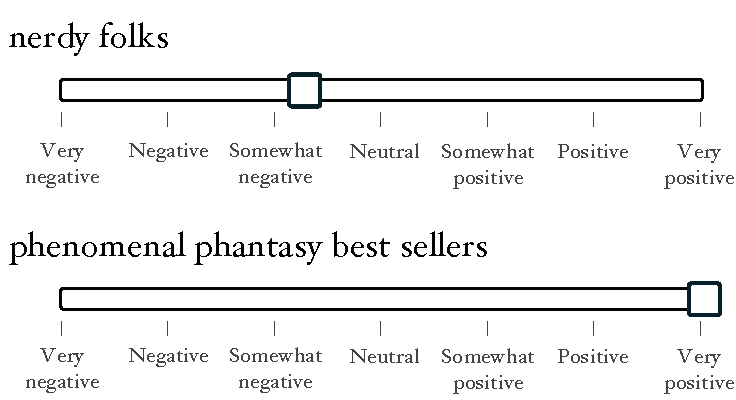
\includegraphics[height=5.5cm]{tramos-polaridad}
\caption[Escala de valoración del sentimiento en Penn Sentiment Treebank]{Escala de valoración del sentimiento empleada en el proyecto Penn Sentiment Treebank de la Universidad de Pennsylvania \citep{Socher2014}}
\label{fig:tramos-polaridad}
\end{figure}


En las páginas dedicadas a opiniones de productos en general como \nombre{Ciao!}\footnote{\url{http://www.ciao.es/}}, o más específicamente para críticas de cine como \nombre{FilmAffinity}\footnote{\url{http://www.filmaffinity.com/}}, se suele proporcionar al usuario un formulario para introducir un texto con su crítica, y además un elemento para que etiquete su valoración, bien en una escala de puntuación o bien mediante estrellitas.

\begin{figure}[htbp]
\centering
\includegraphics[width=0.95\textwidth]{filmaffinity}
\caption[Introducción de la valoración en FilmAffinity]{En FilmAffinity han optado por el desplegable de 1 a 10 puntos etiquetados para introducir la valoración.}
\label{fig:filmaffinity}
\end{figure}

\begin{figure}[htbp]
\centering
\includegraphics[width=0.7\textwidth]{ciao}
\caption[Introducción de la valoración en ciao.es]{Introducción de la valoración en ciao.es, con estrellitas.}
\label{fig:ciao}
\end{figure}

En este tipo de documentos es fácil determinar cuál es la polaridad del texto de la crítica, pues tenemos disponible además un campo de tipo numérico o enumerado (numérico en el sentido de ser inmediatamente procesable por la máquina, sin mayor tratamiento que quizás un cambio de escala o conversión de tipo entero a coma flotante) con la valoración, y podemos asociar valoraciones altas con polaridad buena o muy buena, y las valoraciones bajas con polaridad mala o muy mala. Las valoraciones medias se asociarían a comentarios cuya polaridad del sentimiento será neutra.

\section{Motivación}

Con el amplio uso de las plataformas de twitter y Facebook, los consumidores de productos y servicios pueden criticar abiertamente mediante un comentario a las marcas de las empresas cuyos productos han gustado o no. En la vida virtual, al igual en la vida real, las personas comentamos con nuestros amigos, y recomendamos o no recomendamos estos productos, contribuyendo con nuestras experiencias a mejorar o empeorar la \nombrebf{reputación de las marcas.}\index{reputación!de marca}

Twitter se ha consolidado de esta manera como una forma digital de boca-a-boca \citep{Jansen2009}, pero con mayores posibilidades de alcanzar un gran impacto (o \nombrebf{viralidad}\index{viralidad}) al distribuirse mediante la red global de Internet, y potencialmente llegar a gran cantidad de público. Es más, por nuestra naturaleza, tendemos a reproducir la mala publicidad de un compañía con mayor asiduidad que la buena publicidad, por eso las empresas deben estar presentes en las redes sociales y monitorear su \nombrebf{reputación online}\index{reputación!online} \citep{Leiva2012}.

